\chapter{Using the function space objects}
In this chapter, we show how to use the function space 
objects. These objects are intended to interpret a 
given field. In particular, by using them on a given 
field, we equip the field with the communication pattern 
(thus the Field knows about parallelism), and it allows 
some simple operations on the field. The function space 
objects that will be presented in this chapter are the 
following three:
%
\begin{itemize}
\item \inltc{NodeColumns}: It relates a given field to the underlying 
mesh, thus enabling the field to parallel communication. 
It also allows some simple operations on the Field, such 
as calculating minimum and maximum values, going from a 
local (to a parallel partition) to a global indexing and 
viceversa, etc.
\item \inltc{StructuredColumns}: It relates 
a given field to the underlying structured grid, thus enabling 
the field to parallel communication. It also allows similar 
operations as the \inltc{NodeColumns} function space, such as going 
from a local to a global indexing and viceversa.
\item \inltc{Spectral}: It allows the spectral representation 
of a Field (no relation to a grid or a mesh here!). The 
parallelisation in this case is achieved through the \inlsh{Trans} 
library.
\end{itemize}
%
For each of the function spaces presented in the following, 
we show both the C++ and Fortran version. 

\section{NodeColumns}
For this example, given the length of the code, we divide the code
listings into four different pieces, each of which will highlight 
different functionalities of the function space.

\subsection{C++ version}
%
\begin{description}
%
\item \underline{Construction of Fields}\\[0.5em]
%
The \lista{code-nodes-C-1} shows how to construct the function space 
\inltc{nodes} of type \inltc{NodeColumns} starting from a mesh.
In particular, we first initialize 
the \Atlas library and we define a global structured grid (see lines 
21, 24 and 25). Using this grid, we then construct the mesh (see 
lines 28 and 29) and we get the number of nodes of the mesh (see line 
33). On line 36, we define another integer that is used to construct 
three-dimensional fields if necessary. Specifically, this integer 
is intended to constitute the number of vertical levels required. 
Finally, on lines 39 and 40, we define the function space \inltc{nodes}.
Note that we pass two arguments here: the first is the mesh, while the 
second is the halo. A halo is defined as an extra layer of ghost elements
that is required, for instance, to calculated derivatives when a larger 
stencil is needed. In this case, we just asked for one extra layer of 
ghost elements (i.e. \inltc{Halo(1)}). 
Using the function space \inltc{nodes} just generated, we create 
various fields to highlight the different existing possibilities.

From line 43 to 46, we define two scalar fields (e.g. pressure, 
wind velocity magnitude, etc.). The first field is two-dimensional 
since it does not specify any vertical level. In addition, its 
dimensions automatically correspond to the number of nodes present 
in the mesh (i.e. we do not have to specify its dimensions!), because 
the field is constructed using the function space. Also, by using the 
function space, we automatically enable the field to parallel computation.

From line 47 to 50, we define two vector fields (e.g. wind velocity, etc.).
Again, the first field is purely two-dimensional, while the second contains 
the vertical direction through the parameter \inltc{nb\_levels}, that represents
the number of vertical levels. 

Finally, from line 51 to 54, we show an example on how to construct 
two tensor fields, the first two-dimensional and the second three-dimensional.
The same observations done before for scalar and vector fields hold 
also in this case.
%
\lstinputlisting[caption=Functionspace NodeColumns usage (1) using C++, 
style=CStyle, label=code-nodes-C-1, firstline=1,lastline=55]{NodeColumns.cc}
%
%
\item \underline{Definition/visualization of a scalar Field}\\[0.5em]
%
%
In \lista{code-nodes-C-2}, we show the effective construction 
of a scalar field. We use the same function adopted in \sect{sect:grid-fields}, 
however, in this case, the function is not defined on a grid but 
the mesh through the function space \inltc{nodes}. This also allows 
us to visualize the function in gmsh.

From line 3 to 8, we define some variables needed for the function 
that will be generated. On line 11, we define the \inltc{ArrayView} 
object on the two-dimensional scalar field defined in \lista{code-nodes-C-1}.
On line 12, we extract the implicitly defined \inltc{lonlat} object 
- this step is particularly important since allows us to have access 
to all the coordinates of the nodes in our mesh, order in a 'lonlat
fashion' (where the first dimension, 0, represents the longitudes, 
while the second, 1, represents the latitudes).	
From line 14 to 28, we define the function, a Gaussian-type (hill) 
function - note that the function is now defined on the number of 
nodes of the mesh (not on the number of points of the grid as in 
\sect{sect:grid-fields}!)
%
\begin{warningbox}
Note that the number of points of a grid is different from the number 
of nodes of a mesh!
\end{warningbox}
%
From line 31 to 34, we finally write the mesh and the field in a gmsh 
format, so that we can visualize it!
%
\lstinputlisting[caption=Functionspace NodeColumns usage (2) using C++, 
style=CStyle, label=code-nodes-C-2, firstline=55,lastline=89]{NodeColumns.cc}
%
%
\item \underline{Parallel management}\\[0.5em]
%
In \lista{code-nodes-C-3}, we show some operations related to the 
parallel behaviour of the function space. One of the most important
operations from this perspective is \inltc{HaloExchange} (see line 3). 
This operation allows the correct exchange of information across different 
parallel partitions, when, for instance, calculating derivatives.
A useful command to verify that this operation (or other operations) 
has not corrupted the data is the one reported on line 4, \inltc{checksum}.
This prints a unique identifier for the object that is being passed 
as an argument. If anything in the object changes, this identifier 
will also change, permitting the identification of a possible unwanted 
data corruption. Note also that when printing to the screen this identifier,
we access the MPI rank through \inltc{eckit}.

On line 8, we define a global field, \inltc{field\_global}. 
This, even if the job we are running is parallel, is defined on one task 
only. A global field can be particularly useful for input/output purposes!
Note also that the construction of the global field is based on the existing 
scalar field - i.e. the global field assumes the same characteristics of 
the scalar field, with the only exception that it is defined on one task
only.

On line 11, we apply the \inltc{gather} operation to the global field.
Note that the first argument is the input (in our case \inltc{field\_scalar1}),
while the second argument is the output (in our case \inltc{field\_global}).

We successively print to the screen the number of local mesh nodes 
per parallel partition, the number of points of the grid and the 
number of nodes of the global field.

On line 24, we perform the opposite of the gather operation, 
\inltc{scatter}. As for the \inltc{gather} operation, the 
first argument is the input and the second the output.

From line 27 to 29, we perform an additional \inltc{HaloExchange}, 
and check the integrity of our \inltc{field\_scalar1} after all the 
operations performed using it! 
Finally, from line 32 to 36, we show how \inltc{checksum} can be applied 
also to the \inltc{FieldSet} object.

%
\lstinputlisting[caption=Functionspace nodes usage (3) using C++, 
style=CStyle, label=code-nodes-C-3, firstline=89,lastline=125]{NodeColumns.cc}
%
%
\item \underline{Simple operations}\\[0.5em]
%
In \lista{code-nodes-C-4}, we show some simple operations that 
can be performed using the \inltc{nodes} function space. Specifically, 
on lines 8 and 9 we compute the minimum and maximum values of our 
\inltc{field\_scalar1} - note that the function space knows about 
the parallelisation, therefore there is no need to do anything 
else to obtain the correct minimum and maximum values. This will
also be true for the other operations described below.

On lines 14 and 15, we again calculate the minimum and the maximum 
values of our field but, in this case, we also retrieve the position 
of these values through the global index of the mesh nodes.

On line 22 and 27, we calculate the sum of all the values of our 
field present in the mesh. The two approaches should return the 
same number except for possible round-off errors related to the 
mesh partitioning.

Finally, on line 32 and 36, we compute the mean value of our
field and its standard deviation. Note that the mean and the 
standard deviation are normalised with respect to the total 
number of nodes present in the mesh.

It is also important to observe that we have used a different 
approach than \inltc{cout} to print the values of the quantities 
just calculated to the screen. In particular, we used the 
\inltc{Log::Info()} utility of \Atlas, that will be better 
explained in section \parte{s:utilities-logging}, of this user-guide.
On line 42, we finalize the library as usual.
%
\lstinputlisting[caption=Functionspace nodes usage (4) using C++, 
style=CStyle, label=code-nodes-C-4, firstline=125,lastline=166]{NodeColumns.cc}
%
\end{description}
%
It is now possible to run this simple program by using 
a command-line argument representing the keyword that 
identifies an \Atlas predefined grid.  For instance, 
we can execute the following command line
%
\begin{lstlisting}[style=BashStyle]
./atlas_c-NodeColumns --grid O128
\end{lstlisting}
% 
This will produce an octahedral reduced Gaussian grid 
with 128 latitudes on one hemisphere (i.e. 256 latitudes 
in total), that is then used to generate the mesh and the 
\inltc{nodes} function space. These two will then be used 
to construct our Gaussian-type (hill) scalar field.
The mesh and the field are then written into two \inlsh{.msh}
files. These can be easily opened using Gmsh and they should 
look like \fig{fig:fs_nodes-C}.
%
\begin{figure}%
\centering
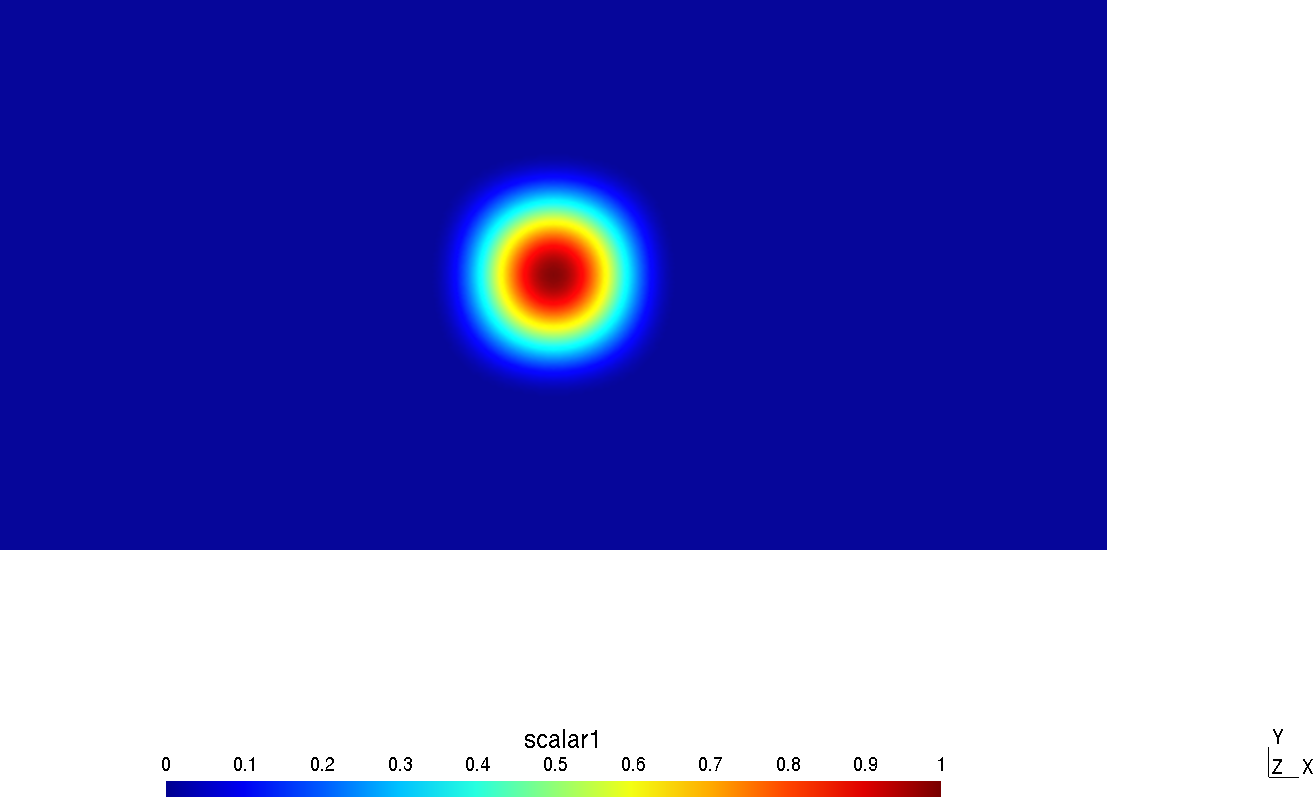
\includegraphics[width=0.75\textwidth]{imgs/O128-field.png}
\caption{Gaussian-type field visualised in Gmsh}%
\label{fig:fs_nodes-C}%
\end{figure}
%
It will also print to the screen the following output:
%
\begin{lstlisting}[style=BashStyle]
[0] (2016-02-11 T 19:24:05) (I) -- writing mesh to gmsh file mesh.msh
[0] (2016-02-11 T 19:24:05) (I) -- writing field partition \
to gmsh file ./mesh_info.msh
[0] (2016-02-11 T 19:24:05) (I) -- writing field partition...
[0] (2016-02-11 T 19:24:05) (I) -- writing field scalar1 \
to gmsh file scalar1.msh
[0] (2016-02-11 T 19:24:05) (I) -- writing field scalar1...
de6c4b5f15bde3b75e3fe927a0e4904c
local nodes         = 70912
grid points          = 70144
field_global.shape(0) = 70144
de6c4b5f15bde3b75e3fe927a0e4904c
9d3b18735c8f114cf4f033204db73e78
[0] (2016-02-11 T 19:24:05) (I) -- min: 0
[0] (2016-02-11 T 19:24:05) (I) -- max: 0.99981
[0] (2016-02-11 T 19:24:05) (I) -- min: 0,  global_id = 1
[0] (2016-02-11 T 19:24:05) (I) -- max: 0.99981,  global_id = 34809
[0] (2016-02-11 T 19:24:05) (I) -- sum: 2872.24, nb_nodes = 70144
[0] (2016-02-11 T 19:24:05) (I) -- oi_sum: 2872.24, nb_nodes = 70144
[0] (2016-02-11 T 19:24:05) (I) -- mean: 0.0409478, nb_nodes = 70144
[0] (2016-02-11 T 19:24:05) (I) -- mean = 0.0409478,  \
std_deviation: 0.1496,  nb_nodes: 70144
\end{lstlisting}
%
In the first few lines, we note that the code informs us that it is 
writing the mesh into gmsh format as well as the field in gmsh format.
Successively, we print the first \inltc{checksum}, that is a string, 
the number of local (to partition) nodes, the total number of grid 
points and the number of entries present in \inltc{field\_global}. 
Note how, for this non-parallel example the number of mesh points 
differs from the number of grid points as mentioned earlier. We 
then print the other two \inltc{checksum}, the first of them is 
identical to the one printed previously - i.e. \inltc{field\_scalar1} 
has not been corrupted! - while the second is different since it 
refers to a different object - i.e. it refer to \inltc{FieldSet}.
Finally, on the last few lines we plot the various minimum, maximum, 
summation, average and standard deviation calculated using the \inltc{nodes}
function space operations.
Note the additional verbosity of the \inltc{Log::Info()} \Atlas utility!

You can now try to generate different meshes and run it in parallel!



\subsection{Fortran version}
%
\begin{description}
%
\item \underline{Construction of Fields}\\[0.5em]
%
The \lista{code-nodes-F-1} shows how to construct the function space 
\inltc{nodes} starting from a mesh. In the first few lines, we define 
the variables needed for this example - note in particular the definition 
of \inltf{atlas\_functionspace\_NodeColumns} and \inltf{atlas\_mesh\_Nodes}.
We then create a structured grid (see lines 48 and 49) and the associated 
mesh (see lines 52 and 53).
On line 45 we initialize the library as usual, while, on line 56, 
we define the \inltf{nodes} function space - note that we pass two 
arguments here: the first is the mesh, while the second is the halo. 
A halo is defined as an extra layer of ghost elements that is required, 
for instance, to calculate derivatives when a larger stencil is needed. 
In this case, we just asked for one extra layer of ghost elements (i.e. 
\inltf{halo\_size = 1}). 

Using the function space \inltf{nodes} just generated, we create 
various fields to highlight the different existing possibilities.

From line 59 to 62, we define two scalar fields (e.g. pressure, 
wind velocity magnitude, etc.). The first field is two-dimensional 
since it does not specify any vertical level. In addition, its 
dimensions automatically correspond to the number of nodes present 
in the mesh (i.e. we do not have to specify its dimensions!), because 
the field is constructed using the function space. Also, by using the 
function space, we automatically enable the field to parallel computation.

From line 63 to 66,  we define two vector fields (e.g. wind 
velocity, etc.). Again, the first field is purely two-dimensional, 
while the second contains the vertical direction through the parameter 
\inltf{nb\_levels}, that represents the number of vertical levels. 

Finally, from line 67 to 70, we show an example on how to construct 
two tensor fields, the first two-dimensional and the second three-dimensional. 
The same observations done before for scalar and vector fields hold 
also in this case.
%
\lstinputlisting[caption=Functionspace atlas\_functionspace\_NodeColumns usage (1) using Fortran, 
style=FStyle, label=code-nodes-F-1, firstline=1,lastline=71]{NodeColumns.F90}
%
%
\item \underline{Definition/visualization of a scalar Field}\\[0.5em]
%
%
In \lista{code-nodes-F-2}, we show the effective construction 
of a scalar field. We use the same function adopted in \sect{sect:grid-fields}, 
however, in this case, the function is not defined on a grid but 
the mesh through the function space \inltc{nodes}. This also allows 
us to visualize the function in gmsh.

On lines 4 and 5, we define the number of nodes of the mesh using 
the \inltf{nodes} function space object.

On line 8, we initialize the pointer \inltf{scalar1} associated
to the two-dimensional \inltf{field\_scalar1} object defined in 
\lista{code-nodes-C-1}.
On lines 9 and 10, we extract the implicitly defined \inltc{lonlat} 
object - this step is particularly important since allows us 
to have access to all the coordinates of the nodes in our mesh, 
ordered in a 'lonlat fashion' (where the first dimension, 1, 
represents the longitudes, while the second, 2, represents 
the latitudes).	From line 12 to 24, we define the function, 
a Gaussian-type (hill) function - note that the function 
is now defined on the number of nodes of the mesh (not on 
the number of points of the grid as in \sect{sect:grid-fields}!)
%
\begin{warningbox}
Note that the number of points of a grid is different from 
the number of nodes of a mesh!
\end{warningbox}
%
On lines 27 and 28, we finally write the mesh and the field 
in a gmsh format, so that we can visualize it!
%
\lstinputlisting[caption=Functionspace atlas\_functionspace\_NodeColumns usage (2) using Fortran, 
style=FStyle, label=code-nodes-F-2, firstline=71,lastline=99]{NodeColumns.F90}
%
%
\item \underline{Parallel management}\\[0.5em]
%
In \lista{code-nodes-F-3}, we show some operations related to the 
parallel behaviour of the function space. One of the most important
operations from this perspective is \inltf{halo\_exchange} (see line 3). 
This operation allows the correct exchange of information across different 
parallel partitions, when, for instance, calculating derivatives.
A useful command to verify that this operation (or other operations) 
has not corrupted the data is the one reported on line 5, \inltc{checksum}.
This prints a unique identifier for the object that is being passed 
as an argument. If anything in the object changes, this identifier 
will also change, permitting the identification of a possible unwanted 
data corruption. Note also that when printing to the screen this identifier,
we access the MPI rank through the \inltf{atlas\_mpi\_rank()} function.

On line 11, we define a global field, \inltf{field\_global}. 
This, even if the job we are running is parallel, is defined on one task 
only. A global field can be particularly useful for input/output purposes!
Note also that the construction of the global field is based on the existing 
scalar field - i.e. the global field assumes the same characteristics of 
the scalar field, with the only exception that it is defined on one task
only.

On line 14, we apply the \inltf{gather} operation to the global field.
Note that the first argument is the input (in our case \inltf{field\_scalar1}),
while the second argument is the output (in our case \inltf{field\_global}).

We successively print to the screen the number of local mesh nodes 
per parallel partition, the number of points of the grid and the 
number of nodes of the global field.

On line 22, we perform the opposite of the gather operation, 
\inltf{scatter}. As for the \inltf{gather} operation, the 
first argument is the input and the second is the output.

On lines 25 and 26, we perform an additional \inltf{halo\_exchange}, 
and check the integrity of our \inltf{field\_scalar1} after 
all the operations performed using it! 
Finally, from line 33 to 35, we show how \inltf{checksum} 
can be applied also to an \inltf{atlas\_FieldSet} object.

%
\lstinputlisting[caption=Functionspace atlas\_functionspace\_NodeColumns usage (3) using Fortran, 
style=FStyle, label=code-nodes-F-3, firstline=99,lastline=137]{NodeColumns.F90}
%
%
\item \underline{Simple operations}\\[0.5em]
%
In \lista{code-nodes-F-4}, we show some simple operations that 
can be performed using the \inltf{nodes} function space. Specifically, 
on lines 5 and 6 we compute the minimum and maximum values of our 
\inltf{field\_scalar1} - note that the function space knows about 
the parallelisation, therefore there is no need to do anything 
else to obtain the correct minimum and maximum values. This will
also be true for the other operations described below.

On lines 12 and 15, we again calculate the minimum and the maximum 
values of our field but, in this case, we also retrieve the position 
of these values through the global index of the mesh nodes.

On lines 20 and 21, we calculate the sum of all the values of our 
field present in the mesh. The two approaches should return the 
same number except for possible round-off errors related to the 
mesh partitioning.

Finally, on lines 26 and 31, we compute the mean value of our
field and its standard deviation. Note that the mean and the 
standard deviation are normalised with respect to the total 
number of nodes present in the mesh.

It is also important to observe that we have used a different 
approach than the standard \inltc{write} to print the values 
of the quantities just calculated to the screen. In particular, 
we used the \inltf{atlas\_log} utility of \Atlas, that will 
be better explained in section \parte{s:utilities-logging}, of this user-guide.

Note also that from line 38 to line 48, we destroy all the objects
of created in the program in order to release the memory and on 
line 50 we finalize the \Atlas library.
%
\lstinputlisting[caption=Functionspace atlas\_functionspace\_NodeColumns usage (4) using Fortran, 
style=FStyle, label=code-nodes-F-4, firstline=137,lastline=188]{NodeColumns.F90}
%
\end{description}
%
It is now possible to run this simple program by using 
a command-line argument representing the keyword that 
identifies an \Atlas predefined grid.  For instance, 
we can execute the following command line
%
\begin{lstlisting}[style=BashStyle]
./atlas_f-NodeColumns --grid O128
\end{lstlisting}
% 
This will produce an octahedral reduced Gaussian grid 
with 128 latitudes on one hemisphere (i.e. 256 latitudes 
in total), that is then used to generate the mesh and the 
\inltc{nodes} function space. These two will then be used 
to construct our Gaussian-type (hill) scalar field.
The mesh and the field are then written into two \inlsh{.msh}
files. These can be easily opened using Gmsh and they should 
look like \fig{fig:fs_nodes-F}.
%
\begin{figure}%
\centering
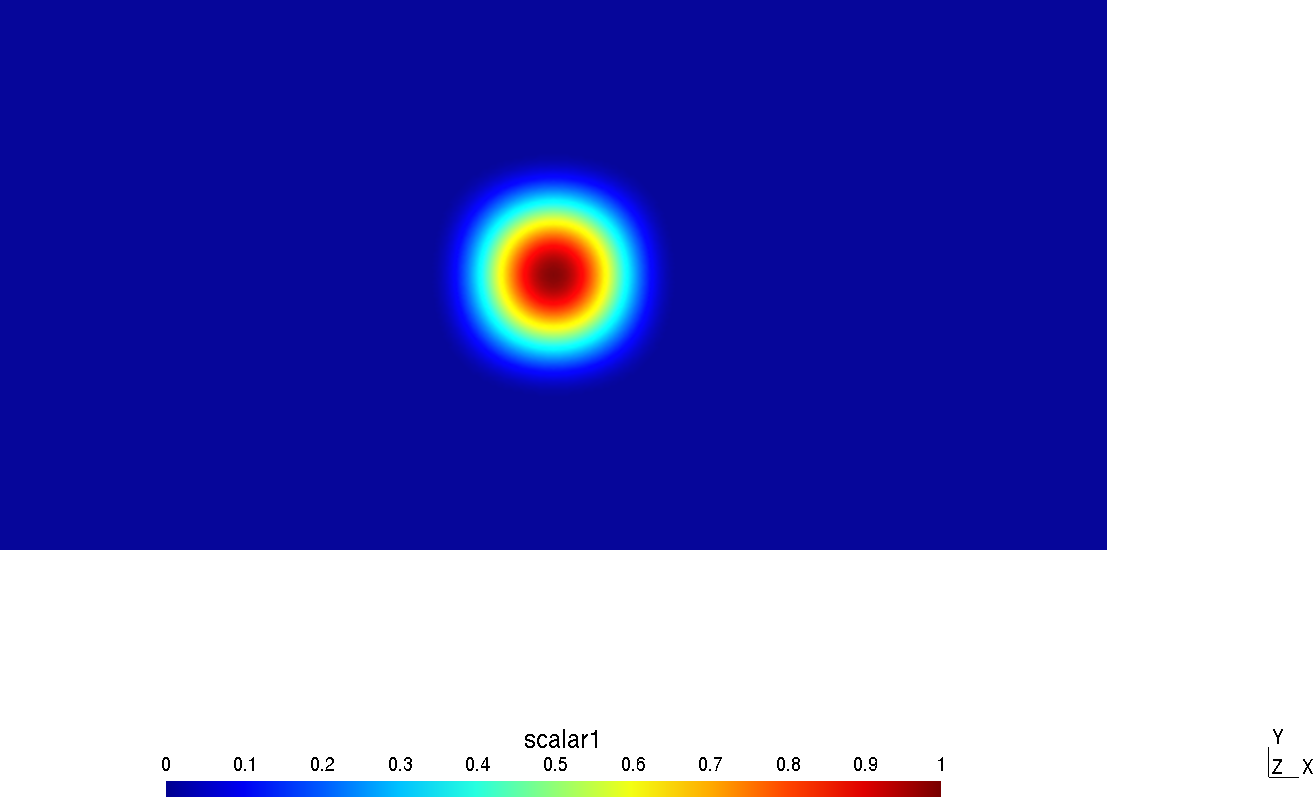
\includegraphics[width=0.75\textwidth]{imgs/O128-field.png}
\caption{Gaussian-type field visualised in Gmsh}%
\label{fig:fs_nodes-F}%
\end{figure}
%
It will also print to the screen the following output:
%
\begin{lstlisting}[style=BashStyle]
[0] (2016-02-12 T 15:41:33) (I) -- Looking for \ 
MeshGeneratorFactory [Structured]
[0] (2016-02-12 T 15:41:34) (I) -- writing mesh \ 
to gmsh file mesh.msh
[0] (2016-02-12 T 15:41:34) (I) -- writing field \ 
field_scalar1 to gmsh file scalar1.msh
[0] (2016-02-12 T 15:41:34) (I) -- writing field \
field_scalar1...
de6c4b5f15bde3b75e3fe927a0e4904c
local nodes          =        70912
grid points          =        70144
field_global.shape(1) =        70144
de6c4b5f15bde3b75e3fe927a0e4904c
9d3b18735c8f114cf4f033204db73e78
[0] (2016-02-12 T 15:41:34) (I) --  min =    0.0000000000000000 \      
max =   0.99981015482709013
[0] (2016-02-12 T 15:41:34) (I) --  min =    0.0000000000000000 \ 
gidx =                     1
[0] (2016-02-12 T 15:41:34) (I) --  max =   0.99981015482709013 \
gidx =                 34809
[0] (2016-02-12 T 15:41:34) (I) --  sum =    2872.2433544940809 \      
oisum =    2872.2433544940809
[0] (2016-02-12 T 15:41:34) (I) --  mean =    4.0947812421505490E-002
[0] (2016-02-12 T 15:41:34) (I) --  mean =    4.0947812421505490E-002
[0] (2016-02-12 T 15:41:34) (I) --  stddev =   0.14959959397019881

\end{lstlisting}
%
In the first few lines, we note that the code informs us that it is 
writing the mesh into gmsh format as well as the field in gmsh format.
Successively, we print the first \inltf{checksum}, that is a string, 
the number of local (to partition) nodes, the total number of grid 
points and the number of entries present in \inltf{field\_global}. 
Note how, for this non-parallel example the number of mesh points 
differs from the number of grid points as mentioned earlier. We 
then print the other two \inltf{checksum}, the first of them is 
identical to the one printed previously - i.e. \inltf{field\_scalar1} 
has not been corrupted! - while the second is different since it 
refers to a different object - i.e. it refer to \inltf{atlas\_FieldSet}.
Finally, on the last few lines we plot the various minimum, maximum, 
summation, average and standard deviation calculated using the \inltf{nodes}
function space operations.
Note the additional verbosity of the \inltf{atlas\_log} \Atlas utility!

You can now try to generate different meshes and run it in parallel!


\section{StructuredColumns}
\section{Spectral}

